% 1991 年上海卷第 14 题：y=x^{-1/3} 的图象选择（依固定扫描页重绘，只画拓扑与标号，不按比例）
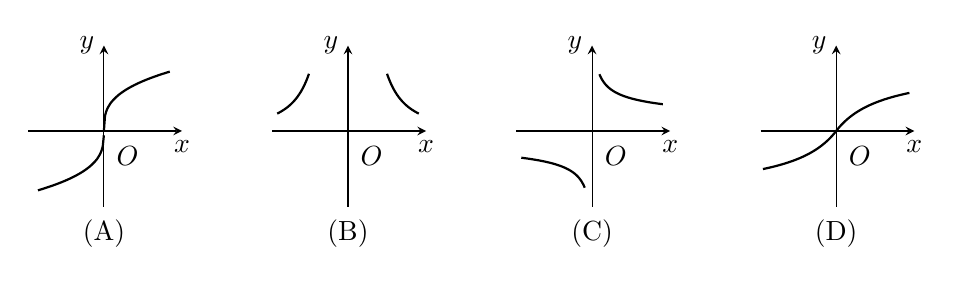
\begin{tikzpicture}[>=stealth,scale=0.62]
  % (A) 过原点、两侧都单调增，原点处切线竖直（y=x^{1/3} 型）
  \begin{scope}[shift={(0,0)}]
    \draw[->] (-1.55,0)--(1.60,0) node[below] {$x$};
    \draw[->] (0,-1.55)--(0,1.75) node[left] {$y$};
    \node[below right] at (0.06,-0.12) {$O$};
    \draw[thick,domain=0:1.35,samples=60] plot (\x,{1.10*(\x)^(0.3333)});
    \draw[thick,domain=-1.35:0,samples=60] plot (\x,{-1.10*(-\x)^(0.3333)});
    \node at (0,-2.10) {(A)};
  \end{scope}
  % (B) 两支都在 x 轴上方，各自单调减，y 轴为渐近线（偶函数型）
  \begin{scope}[shift={(5.0,0)}]
    \draw[->] (-1.55,0)--(1.60,0) node[below] {$x$};
    \draw[->] (0,-1.55)--(0,1.75) node[left] {$y$};
    \node[below right] at (0.06,-0.12) {$O$};
    \draw[thick,domain=0.80:1.45,samples=60] plot (\x,{0.75/(\x*\x)});
    \draw[thick,domain=-1.45:-0.80,samples=60] plot (\x,{0.75/(\x*\x)});
    \node at (0,-2.10) {(B)};
  \end{scope}
  % (C) 右支在 x 轴上方单调减，左支在 x 轴下方单调减，y 轴为渐近线（奇函数型）
  \begin{scope}[shift={(10.0,0)}]
    \draw[->] (-1.55,0)--(1.60,0) node[below] {$x$};
    \draw[->] (0,-1.55)--(0,1.75) node[left] {$y$};
    \node[below right] at (0.06,-0.12) {$O$};
    \draw[thick,domain=0.15:1.45,samples=80] plot (\x,{0.62*(\x)^(-0.3333)});
    \draw[thick,domain=-1.45:-0.15,samples=80] plot (\x,{-0.62*(-\x)^(-0.3333)});
    \node at (0,-2.10) {(C)};
  \end{scope}
  % (D) 过原点、单调增，两端趋近水平（有水平渐近线）
  \begin{scope}[shift={(15.0,0)}]
    \draw[->] (-1.55,0)--(1.60,0) node[below] {$x$};
    \draw[->] (0,-1.55)--(0,1.75) node[left] {$y$};
    \node[below right] at (0.06,-0.12) {$O$};
    \draw[thick,domain=0:1.50,samples=60,smooth] plot (\x,{1.30*\x/(1+\x)});
    \draw[thick,domain=-1.50:0,samples=60,smooth] plot (\x,{1.30*\x/(1-\x)});
    \node at (0,-2.10) {(D)};
  \end{scope}
\end{tikzpicture}
